\chapter{Installation}

In this section, we present the installation process for the toolbox.
We present the steps which are required to have a running version of the 
toolbox and presents the several checks which can be performed before 
using the toolbox.

\section{Architecture of the directories}

We suppose that the archive has been unpacked in the "neldermead" 
directory. The following is a short list of the steps which are 
required to setup the toolbox.

\begin{enumerate}
\item build the toolbox : run the \emph{neldermead/builder.sce} script to 
create the binaries of the library, create the binaries 
for the gateway, generate the documentation
\item load the toolbox : run the \emph{neldermead/loader.sce} script to 
load all commands and setup the documentation
\item setup the startup configuration file of your Scilab system so that the toolbox is 
known at startup (see below for details),
\item run the unit tests : run the \emph{neldermead/runtests.sce} script to 
perform all unit tests and check that the toolbox is OK
\item run the demos : run the \emph{neldermead/rundemos.sce} script to 
run all demonstration scripts and get a quick interactive 
overview of its features
\end{enumerate}

The easiest way to setup your Scilab system is to configure the 
startup configuration file so that the toolboxes are known immediately
at startup. The directory where this file is located is stored in the 
Scilab variable \emph{SCIHOME}.
On my Linux system, the Scilab 5.1 startup file is located
in \emph{/home/myname/.Scilab/scilab-5.1/.scilab}. On my Windows system, the Scilab 5.1 startup file is located
in \emph{C:/Users/myname/AppData/Roaming/Scilab/scilab-5.1/.scilab}.
This file is a regular Scilab script which is automatically 
loaded at Scilab's startup. If that file does not already 
exist, create it. Copy the following lines into the \emph{.scilab} file 
and configure the path to the toolboxes, stored in the \emph{SCILABTBX} variable.

\begin{verbatim}
ilib(0);
SCILABTBX="/home/myname/mytoolboxes";
exec(SCILABTBX + filesep() + 'optimbase'+ filesep() + 'loader.sce');
exec(SCILABTBX + filesep() + 'optimsimplex'+ filesep() + 'loader.sce');
exec(SCILABTBX + filesep() + 'neldermead'+ filesep() + 'loader.sce');
\end{verbatim}

The figure \ref{installation:builder.sce} presents the messages
which are generated when the builder of the toolbox is launched.

\begin{figure}[htbp]
\begin{small}
\begin{verbatim}
-->cd neldermead/
 ans  =
 /media/disk/SVN-Scilab/neldermead   
-->exec builder.sce
-->// ====================================================================
-->// Copyright INRIA 2008-2009
-->// Allan CORNET
-->// Simon LIPP
-->// Michael Baudin
-->// This file is released into the public domain
-->// ====================================================================
-->mode(-1);
Building macros...
-- Cr�ation de [neldermeadlib] (Macros) --
genlib: Traitement du fichier: nmplot_display.sci
[...]
genlib: Traitement du fichier: nmplot_configure.sci
genlib: Regenere noms et librairie
Building help...
Construit le document principal dans /media/disk/SVN-Scilab/neldermead/help/en_US
Construction du fichier manuel [javaHelp] dans /media/disk/SVN-Scilab/neldermead/help/en_US. (Veuillez patienter ... cela peut prendre un certain temps)
Generating loader.sce...
\end{verbatim}
\end{small}
\caption{Launch of the builder}
\label{installation:builder.sce}
\end{figure}

The figure \ref{installation:loader.sce} presents the messages
which are generated when the loader of the toolbox is launched.

\begin{figure}[htbp]
\begin{small}
\begin{verbatim}
->exec loader.sce
 
-->// ====================================================================
-->// generated by builder.sce
-->// Copyright INRIA 2008
-->// ====================================================================
-->try
--> getversion('scilab');
-->catch
--> warning('Scilab 5.0 or more is required.');
--> return;
-->end;
-->// ====================================================================
-->root_tlbx = get_absolute_file_path('loader.sce');
-->exec(root_tlbx+'etc\'+'neldermead.start');
 Start Nelder-Mead Toolbox   
 Load macros from :   
 /media/disk/SVN-Scilab/neldermead/macros/   
 Load help   
-->// ====================================================================
-->clear root_tlbx;
-->// ====================================================================
\end{verbatim}
\end{small}
\caption{Launch of the loader}
\label{installation:loader.sce}
\end{figure}

The figure \ref{installation:runtests.sce} presents the messages
which are generated when the unit tests script of the toolbox is launched.

\begin{figure}[htbp]
\begin{verbatim}
-->exec D:\Baudin\ProjetScilab\toolboxes\neldermead\runtests.sce
-->TODO ...
\end{verbatim}
\caption{Launch of the unit tests script}
\label{installation:runtests.sce}
\end{figure}


\section{Configuration}

The directories which are provided in the toolbox 
are presented in figure \ref{installation:neldermeaddirectory}.

\begin{figure}[htbp]
\begin{center}
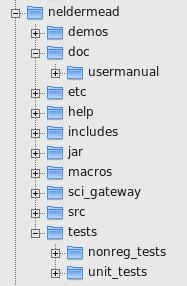
\includegraphics[height=5cm]{installation-directories.png}
\end{center}
\caption{Architecture of the toolbox}
\label{installation:neldermeaddirectory}
\end{figure}

This is an overview of the content of these directories :
\begin{itemize}
\item \emph{neldermead/demos} : demonstration scripts
\item \emph{neldermead/doc} : the Scilab Enhancement Proposal \#21, about Nelder-Mead algorithm
\item \emph{neldermead/doc/usermanual} : the \LaTeX sources of this manual
\item \emph{neldermead/etc} : startup and shutdow scripts for the toolbox
\item \emph{neldermead/help/en\_US/scilab\_en\_US\_help} : html pages of the help
\item \emph{neldermead/jar} : java archive for the help
\item \emph{neldermead/macros} : Scilab macros files *.sci
\item \emph{neldermead/tests} : tests
\item \emph{neldermead/tests/nonreg\_tests} : tests after some bug has been identified
\item \emph{neldermead/tests/unit\_tests} : unit tests
\end{itemize}

\section{Tests}


